\thispagestyle{empty}
\noindent
\includegraphics[width=0.55\textwidth]{bilder/misc/MPIWG_d_WM_4c.eps}
\vspace{20mm}


\noindent This document is the rendition of an TEI-P5 XML document as
a PDF file and was created automatically by a script and Lua\LaTeX. The source is a
transcription of a facsimile along the guidelines designed at the
MPIWG which can be found at \url{https://github.molgen.mpg.de/kthoden/despecs}.

\noindent Some features of the text are highlighted by boxes
\begin{description}
\item[Pagebreaks] If there is a pagenumber on the original page, it is displayed. The original running header of a page occurs to the right of the box.
\item[Figures] The figures themselves are not displayed. If the caption or contents like variables or descriptive elements were typed, they are also displayed in the box.
\item[Missing characters] Missing characters are rendered as ``??'' in a box.
\item[Handwritten text] Handwritten text is not transcribed, but the occurrences are noted.
\item[@] When the character ``@'' occurs in the text, it denotes also an unclear character.
\end{description}

\noindent When proofreading the source, add your corrections by annotating the PDF.

\vfill

\noindent\includegraphics[width=0.13\textwidth]{bilder/misc/by.eps}

\noindent This work is licensed under the Creative Commons Attribution 4.0 International License. To view a copy of this license, visit \url{https://creativecommons.org/licenses/by/4.0/} or send a letter to Creative Commons, PO Box 1866, Mountain View, CA 94042, USA.

\newpage
